\documentclass[crop,tikz]{standalone}
\usepackage{scalerel}

\begin{document}
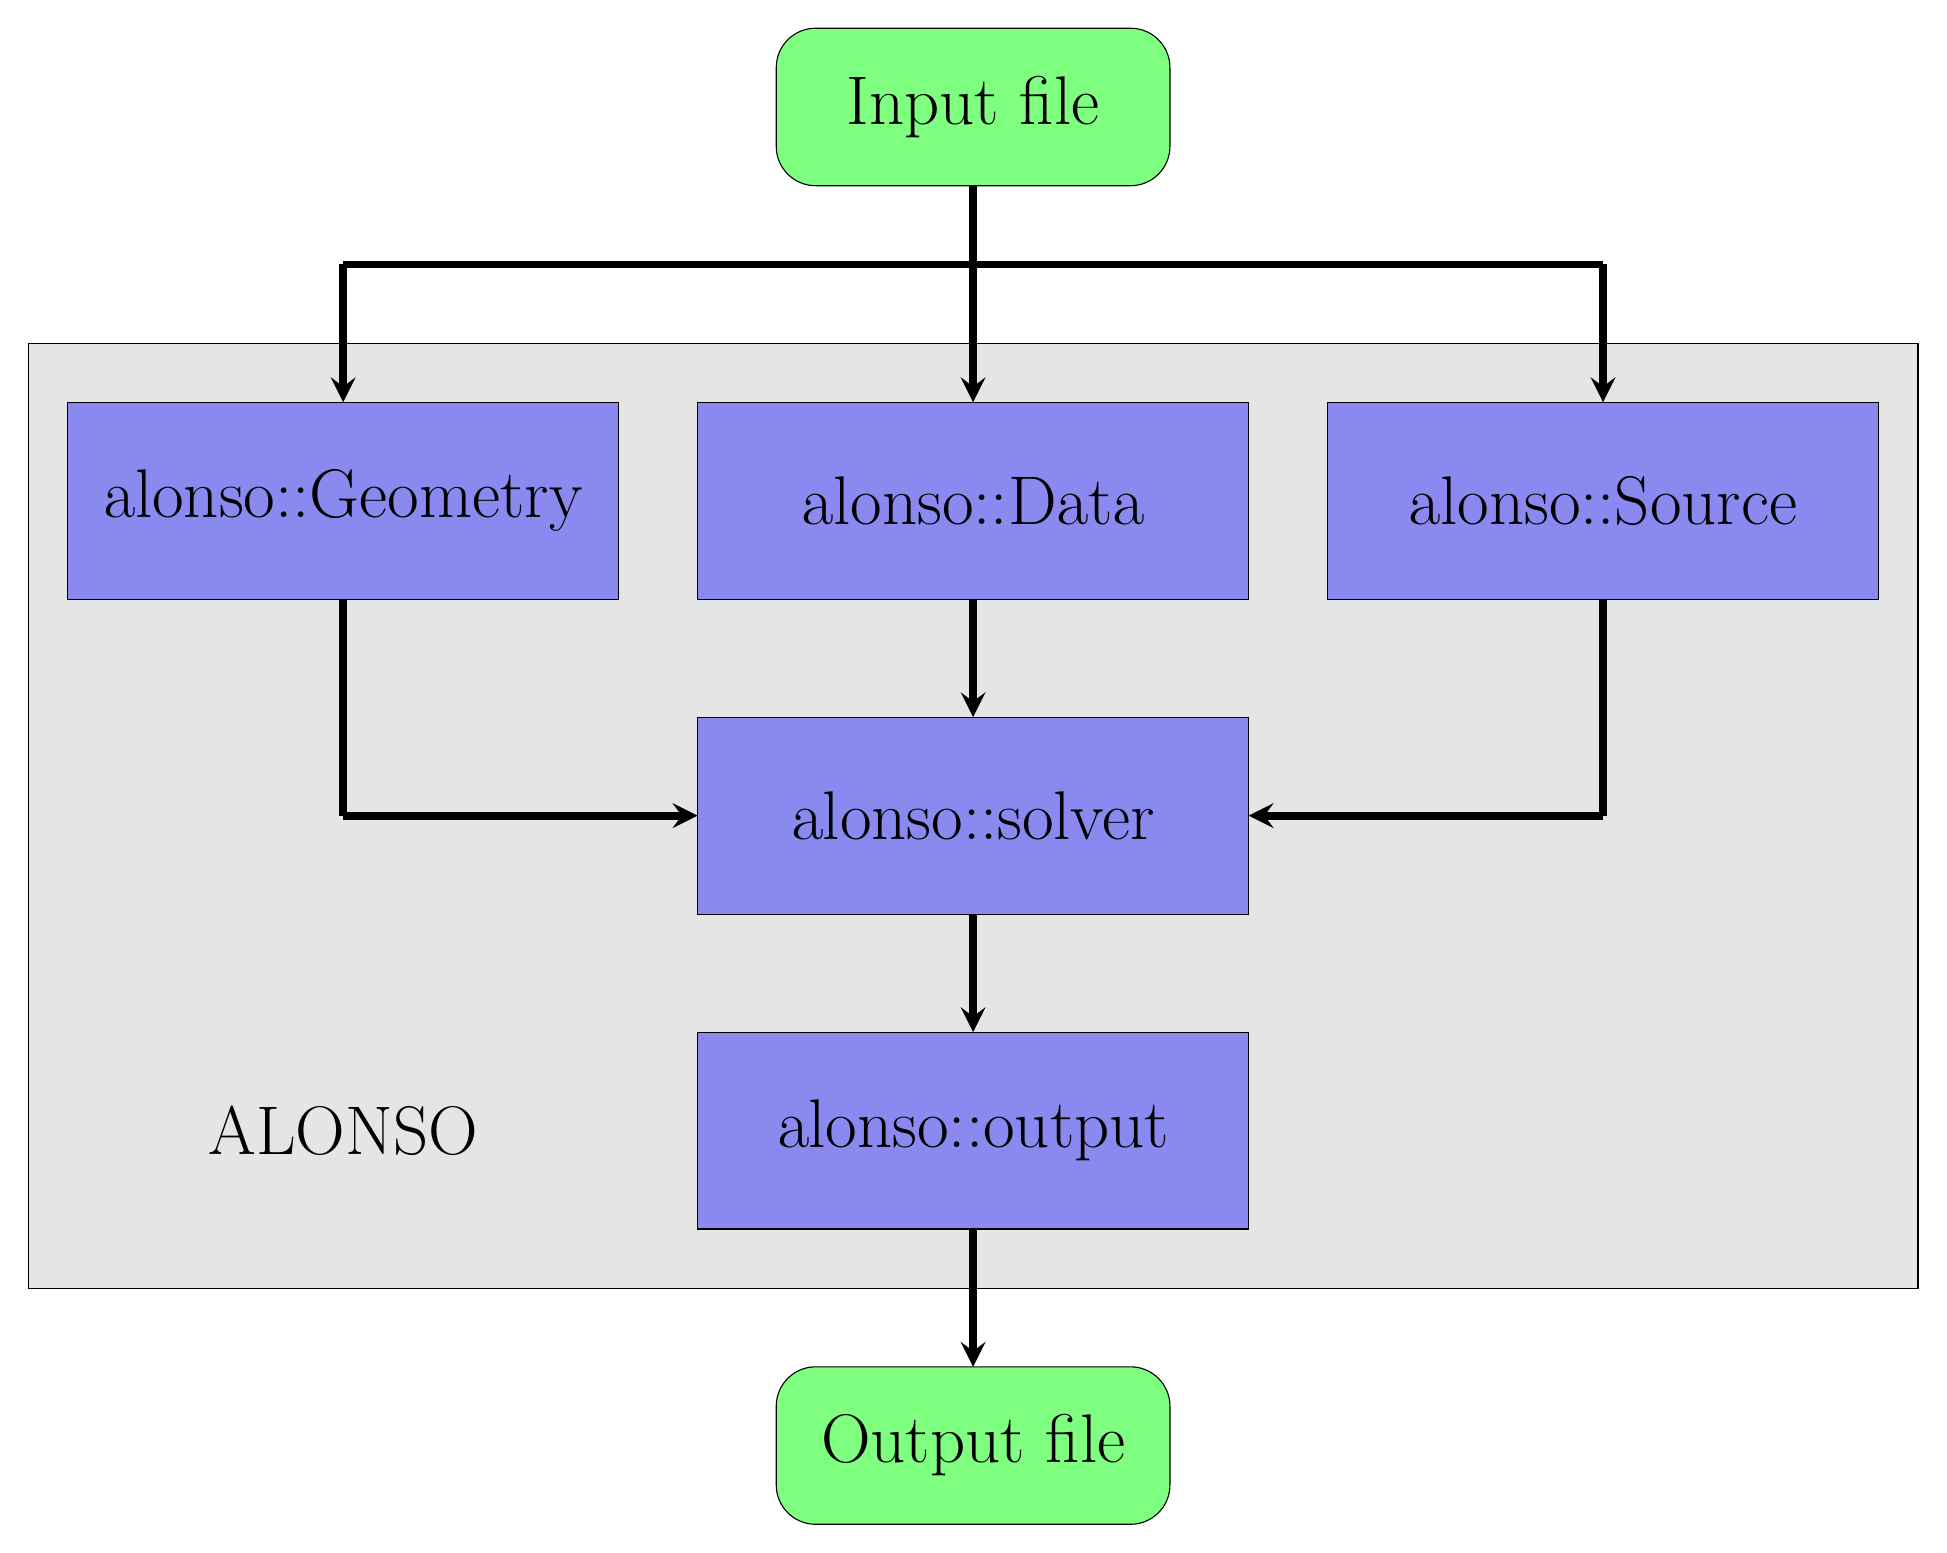
\begin{tikzpicture}
    % ALONSO Code
    \node[draw,
      minimum width=24cm,
      minimum height=12cm,
      fill=lightgray,
      fill opacity=0.4] (PProcess) at (0,-4) {};
      
    % ENDF file
    \node[draw,
      rounded corners=0.5cm,
      minimum width=5cm,
      minimum height=2cm,
      fill=green,
      fill opacity=0.5,
      text opacity = 1] at (0,5){\Huge{Input file}};
      
    % Geometry.hpp
    \node[draw,
      minimum width=7cm,
      minimum height=2.5cm,
      outer sep=0,
      fill=blue,
      fill opacity=0.4,
      text opacity=1] (PProcess) at (-8,0)  {\Huge{alonso::Geometry}};
      
    % Data.hpp
    \node[draw,
      minimum width=7cm,
      minimum height=2.5cm,
      outer sep=0,
      fill=blue,
      fill opacity=0.4,
      text opacity=1] (PProcess) at (0,0)  {\Huge{alonso::Data}};
      
    % Source.hpp
    \node[draw,
      minimum width=7cm,
      minimum height=2.5cm,
      outer sep=0,
      fill=blue,
      fill opacity=0.4,
      text opacity=1] (PProcess) at (8,0)  {\Huge{alonso::Source}};

    % Solver
    \node[draw,
      minimum width=7cm,
      minimum height=2.5cm,
      outer sep=0,
      fill=blue,
      fill opacity=0.4,
      text opacity=1] (PProcess) at (0,-4)  {\Huge{alonso::solver}};

    % Output
    \node[draw,
      minimum width=7cm,
      minimum height=2.5cm,
      outer sep=0,
      fill=blue,
      fill opacity=0.4,
      text opacity=1] (PProcess) at (0,-8)  {\Huge{alonso::output}};
    
    % JSON file
    \node[draw,
      rounded corners=0.5cm,
      minimum width=5cm,
      minimum height=2cm,
      fill=green,
      fill opacity=0.5,
      text opacity = 1] at (0,-12){\Huge{Output file}};
    
    % Draw Arrows
    \draw[-stealth, line width=1mm] (0, 4) -- ( 0.0, 1.25);
    \draw[line width=1mm] (0, 3) -- (-8, 3);
    \draw[-stealth, line width=1mm] (-8, 3) -- (-8, 1.25);
    \draw[line width=1mm] (0, 3) -- ( 8, 3);
    \draw[-stealth, line width=1mm] ( 8, 3) -- ( 8, 1.25);

    \draw[-stealth, line width=1mm] (0, -1.25) -- ( 0,-2.75);
    \draw[line width=1mm] (-8, -1.25) -- (-8,-4);
    \draw[-stealth, line width=1mm] (-8,-4) -- (-3.5,-4);
    \draw[line width=1mm] ( 8, -1.25) -- ( 8,-4);
    \draw[-stealth, line width=1mm] ( 8,-4) -- ( 3.5,-4);

    \draw[-stealth, line width=1mm] (0, -5.25) -- ( 0,-6.75);

    \draw[-stealth, line width=1mm] (0, -9.25) -- ( 0,-11);
    
    % Text labels
    \node at (-8, -8) {\Huge{ALONSO}};
  \end{tikzpicture}
\end{document}